\section{Math Theory}
\label{maththeory}
This section will describe which factors must be known, before any necessary calculations can be performed.

\subsection{Object Trajectory Prediction}
From the time an object is detected, until the projectile can hit it, takes some time. To be able to hit the object, it is necessary to know where it will be at the time of impact. We must therefore be able to predict the trajectory of the object.

If the object moves in an unpredictable pattern, it can be difficult to hit. A predictable parabolic or straight line pattern is almost essential to be able to hit the object. If the object moves in a predictable pattern, it is possible to know where it is at the time of impact.

Calculating the position of an object moving in a straight line is pretty simple. The only factors needed is the position of the object at a specific time, and the speed and direction of the object. If the object moves in a parabolic line, then calculating its position is a bit more difficult, because then you have to solve a quadratic equation.

If the object is flying, or it in other ways are moving up or down, there is a whole other level of complexity in the calculations. The objects movement will then go from a two dimensional plane to a three dimensional space.

\subsection{Projectile Trajectory Analysis}
When the targets position has been predicted, the projectile should be launched and hit the target. To know where to shoot the projectile at, the trajectory of the projectile must be calculated.
The projectiles trajectory will be parabolic\cite{trajectoryanalysis}, thus the calculations needed will be to find the derivative of a quadratic equation.

To know when to launch the projectile, and at which angle, it is necessary to know the speed of the projectile, the distance to the predicted target, and the height difference between the cannon and the target. Once this is known, it is possible to calculate the trajectory that the projectile will have to travel to hit the target, and thus calculate the angle of launch. The projectile will fly in a parabolic trajectory, two different trajectories can hit the same target, \autoref{fig:projectile-trajectory} shows a high angle and a low angle shot.

\begin{figure}[hbtp]
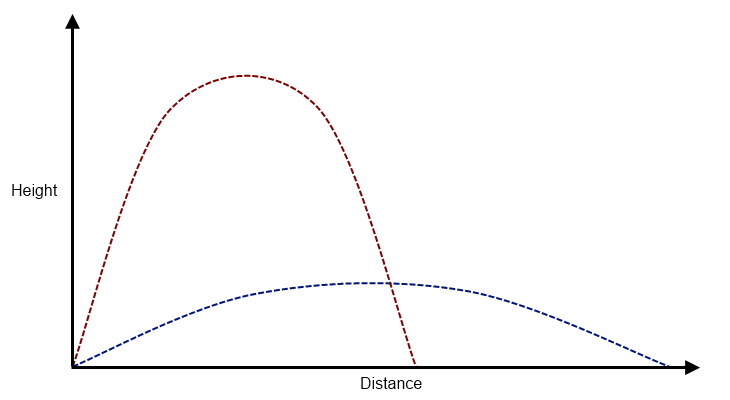
\includegraphics[width=\textwidth]{img/projectile-trajectory-graph.png}
\caption{Example of projectile trajectories.} 
\label{fig:projectile-trajectory} 
\end{figure}

When the angle of launch is known, the only remaining task is to know how much time it takes the projectile to get to the target, and thus when to shoot.

\subsection{Transformation from Kinect Coordinates to Turret}
The Kinect returns coordinates in a rather odd fashion. The depth measurement is measured in an 11 bit int array\cite{kinectdistance}. The distance is thus not measured in a distance of millimeters, but instead in a distance of arbitrary numbers from 0 to 2047. Furthermore, the distance measured is not linear, it is quadratic, meaning that distances close to zero have a higher precision than distances further away.
The width and height of an object is measured with the RGB camera, and is measured in pixels. This measurement cannot directly give coordinates for the object. The pixels are a representation of the Kinects field of  view, which is larger in the horizontal direction than the vertical direction. To find the exact coordinate of an object it is necessary to calculate the angle between the Kinects center and the object, together with the depth it is possible to calculate the coordinate position.